\documentclass[10pt,a4paper]{scrartcl}

\usepackage[ngerman]{babel}			% N�tig f�r deutsche Silbentrennung
\usepackage[ansinew]{inputenc}		% N�tig f�r deutsche Umlaute
\usepackage{scrpage2}				% N�tig f�r Fusszeile
\usepackage{graphicx}				% N�tig f�r eingebettete Bilder
\usepackage{listings}				% N�tig f�r Quelltext-Einbindung
\usepackage{courier}				% N�tig f�r Courier-Font (Quelltext)
\usepackage[bottom=10em]{geometry}	% N�tig f�r Gr�ssenver�nderung Fusszeile
\usepackage{placeins}				% N�tig f�r feste Positionen von Grafiken

\clearscrheadfoot
\pagestyle{plain}

% Geforderte "Formatvorlage" f�r Autoren; Parameter:
% - 1) Vor- & Zuname
% - 2) Matrikelnummer
\newcommand{\autor}[2]{#1, \\ & & Matrikelnummer #2}

% Geforderte "Formatvorlage" f�r Quellcode; Parameter:
% - 1) Sprache des Quellcodes (siehe: https://en.wikibooks.org/wiki/LaTeX/Source_Code_Listings#Supported_languages)
% - 2) Zeilengr�sse (nicht Schriftgr�sse!), Standard: 10
%
% Muss gefolgt werden mit:
% \begin{lstlisting}[frame=single]
% ... Code ...
% end{lstlisting}
\newcommand{\code}[2]{\lstset{language=#1, basicstyle=\fontsize{8}{#2}\selectfont\ttfamily}}


\begin{document}


% ================================================================================
%
%		Titelblatt (Institution, Titel/ Untertitel, Studiengang/ Semester, Autor, Datum, Version)
%
% ================================================================================
\begin{center}
	\LARGE{Hochschule Niederrhein} \\
	\Large{Fachbereich Elektrotechnik und Informatik} \\
	\large{Labor f\"ur Echtzeitsysteme}
\end{center}
\begin{verbatim}







\end{verbatim}
\begin{center}
	\textbf{\huge{Praktikum Echtzeitsysteme}} \\
	\textbf{\LARGE{Termine 1-3}} \\
	\textbf{\Large{B-I-5}}
\end{center}
\begin{verbatim}







\end{verbatim}
\begin{center}
	\begin{tabular}{lll}
		\textbf{Autor:} & & \autor{Tobias Hahnen}{1218710} \\
		& & \autor{Mike Wandels}{1165207} \\
		& & \\
		\textbf{Gruppe:} & & C \\
		& & \\
		\textbf{Datum:} & & \today \\
		& & \\
		\textbf{Version:} & & 1.0.0
	\end{tabular}
\end{center}


\newpage


% ================================================================================
%
%		Inhaltsverzeichnis (automatisch generiert)
%
% ================================================================================
\tableofcontents
\newpage


% ================================================================================
%
%		1) Beschreibung der Aufgabenstellung
%
% ================================================================================
\section{Beschreibung der Aufgabenstellung}

Im Zuge des Praktikums Echtzeitsysteme soll eine Steuerung f\"ur eine Carrerabahn erstellt und erweitert werden, sodass ein Fahrzeug eine Bahn abfahren und ausmessen kann und danach gegen einen Gegner ein Rennen fahren kann.
Diese Steuerung sollte dabei unabh\"angig von Auto, Carrerabahn und der verwendeten Spur sein. \\
Dazu f\"ahrt das Auto vor Rennbeginn die Strecke ab und misst anhand der Zeit, die das Auto durch die Lichtschranken braucht, die L\"ange der einzelnen Elemente und f\"ugt diese einer Liste hinzu.
Es gibt zwei Bahnen mit unterschiedlichen Elementen und einer jeweils anderen Anordnung, daher muss die Steuerung auch das beste aus der Anordnung herausholen. \\
Im anschliessenden Rennen soll sich das Fahrzeug gegen den Gegner behaupten, indem es auf die unterschiedlichen Stati reagiert.
Das heisst, dass die Auslenkung in den Kurven beachtet werden muss sowie die Tatsache, ob sich das Fahrzeug auf der Innen- oder Aussenbahn befindet und bei vorkommenden Gefahrenstellen, ob sich bereits der Gegner darin befindet oder nicht und dementsprechend wartet oder durchf\"ahrt.
Anhand der in den Stati \"ubergebenen Informationen sollte dann auch eine dynamische Geschwindigkeitsanpassung implementiert werden, sodass auf unterschiedlichen Streckenabschnitten unterschiedliche Geschwindigkeiten gefahren werden k\"onnen, um das meiste aus diesen Abschnitten herauszuholen, ohne dass das Fahrzeug aus der Bahn fliegt oder eine Kollision verursacht.


% ================================================================================
%
%		2) Bedienung der Applikation
%
% ================================================================================
\section{Bedienung der Applikation}

Bedient wird die Applikation \"uber die Kommandozeile, indem sie wie folgt aufgerufen wird:

\code{Bash}{10}
\begin{lstlisting}[frame=single]
$ ./race {Geschwindigkeit} {Runden}
\end{lstlisting}

Dabei gibt die \textit{Geschwindigkeit} die zum Start des Rennens an, in der Erkundungsphase f\"ahrt das Fahrzeug in einer anderen. \\
Die \textit{Runden} geben die L\"ange des Rennens an, die Erkundungsphase ist davon unabh\"angig. \\

W\"ahrend des Rennens gibt es einige Ausgaben auf dem Bildschirm, die allerdings nur eine Information angeben, man kann nicht mit dem Programm interagieren, nachdem es gestartet wurde.
Wenn man es allerdings per Keyboard Interrupt (Strg-C) abbricht, stoppt auch das Fahrzeug auf der Strecke.


% ================================================================================
%
%		3) Generierung und Installation
%
% ================================================================================
\section{Generierung und Installation}

Zur Generierung wird das Build-Management-Tool \textit{Make} und die dazugeh\"orige Makefile ben\"otigt.
Ausserdem wird der Compiler \textit{GCC/G++}, die Echtzeitbibliothek \textit{RT} und ein Unixartiges Betriebssystem vorausgesetzt. \\
Die Erstellung des Programms erfolgt \"uber die folgenden Aufrufe des Tools \textit{Make}:

\code{Bash}{10}
\begin{lstlisting}[frame=single]
$ make clean
$ make all
\end{lstlisting}

Danach kann das Programm wie in der Sektion \textit{Bedienung der Applikation} beschrieben aufgerufen werden.

\newpage


% ================================================================================
%
%		4) Skizzierung der L�sung
%
% ================================================================================
\section{Skizzierung der L\"osung}

Die L\"osung zu der gegebenen Aufgabenstellung baut auf dem vorgegebenen Code-Ger\"ust auf. 

\subsection{Verbale Beschreibung der L\"osung}

Das Programm durchl\"auft im Wesentlichen zwei Schritte. \\

Der 1. Schritt ist die Erkundung und Vermessung der Strecke, daf\"ur wird die Art des momentanen Elements durch das erhaltene Statuswort des Carrerabahn-Treibers ermittelt und die L\"ange mithilfe der Durchfahrtszeit und der angegebenen Geschwindigkeit errechnet.
Diese Informationen werden dann in einer Liste f\"ur den zweiten Schritt abgelegt.
Der Schritt ist beendet, sobald das Fahrzeug das Start/ Ziel Element erneut erreicht, danach wartet es auf den Start des Rennens, die durch eine simple Benutzereingabe erfolgt. \\

Der 2. Schritt, das eigentliche Rennen, besteht im Wesentlichen aus zwei Teilen, der eine behandelt unser Fahrzeug und der andere das des Gegners.
Beide laufen in einem separaten Thread, sodass sie beide auf dieselben Ressourcen zugreifen k\"onnen. \\
Der Gegnerthread dient zur \"Uberwachung, an welcher Stelle der Rennbahn sich der Gegner befindet um die Kollisionsstelle fachgerecht zu handhaben.
Daf\"ur wird die Position des Gegners mit einem Zeiger auf das entsprechende Bahnelement gespeichert, sodass es vom Thread, der unser Fahrzeug handhabt, abgerufen werden kann. \\
Der Thread, der unser Fahrzeug steuert, handhabt die gesamte Steuerung, bestehend aus der dynamischen Geschwindigkeitsanpassung, der richtigen Reaktion an der Gefahrenstelle, basierend auf der Position des Gegners, sowie der Erkennung von Auslenkung in Kurven und der damit verbundenen Reaktion auf M\"oglichkeiten, aus der Bahn zu fliegen. \\
Dazu wird das aktuelle, vom Carrerabahn-Treiber eingelesene, Statuswort ausgewertet, welches zuerst auf die Auslenkung getestet wird, was bedeutet, dass sich das Fahrzeug in einer Kurve befindet.
Sollte die Auslenkung zu hoch sein, wird dementsprechend reagiert.
Danach wird das aktuelle Element mit dem des Gegners verglichen, um eine Kollision an der Gefahrenstelle zu vermeiden.
Zuletzt wird die Geschwindigkeit anhand des derzeitigen Elements dynamisch ermittelt und angepasst. \\

Wenn das Rennen beendet wurde, nach der \"ubergebenen Anzahl von Runden, bleibt das Fahrzeug am Start/ Ziel Element stehen und das Programm endet.

\newpage


\subsection{Datenflussdiagramm}

\begin{figure}[h!]
	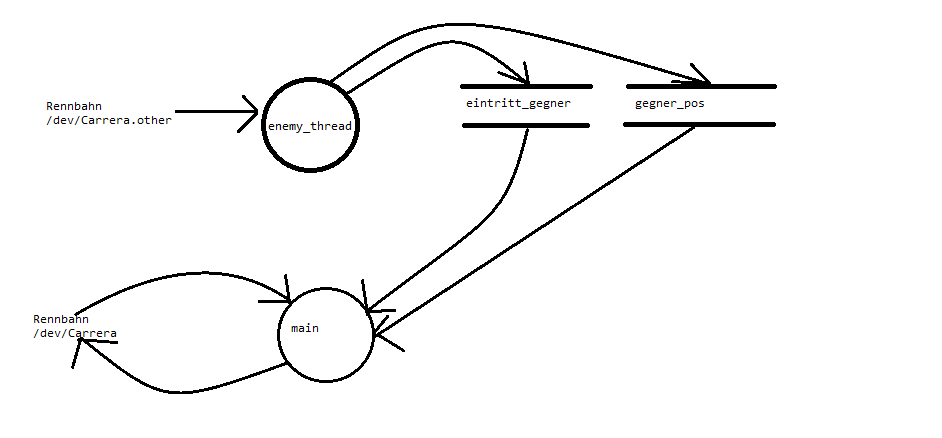
\includegraphics[width=\textwidth]{Datenflussdiagramm.png}
	\caption{Treiber zu Gegnerthread und Mainthread}
\end{figure}
\FloatBarrier

\subsection{Strukturgramme: Mainthread}

\begin{figure}[h!]
	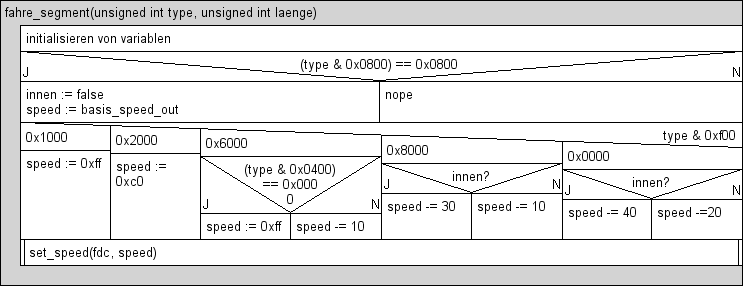
\includegraphics[width=\textwidth]{Diagramm-fahre_segment.png}
	\caption{Funktion: \textit{void fahre\_segment(unsigned int type, unsigned int laenge)}}
\end{figure}
\FloatBarrier

\begin{figure}[h!]
	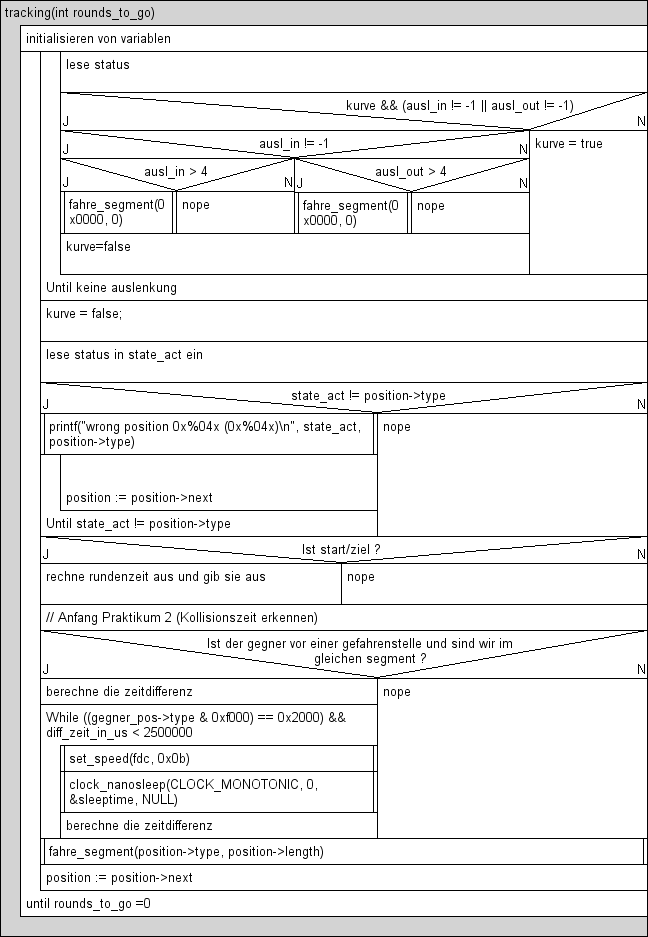
\includegraphics[width=\textwidth]{Diagramm-tracking.png}
	\caption{Funktion: \textit{void tracking(int rounds\_to\_go)}}
\end{figure}
\FloatBarrier

%\subsection{Strukturgramme: Gegnerthread}
%\begin{figure}[h!]
%	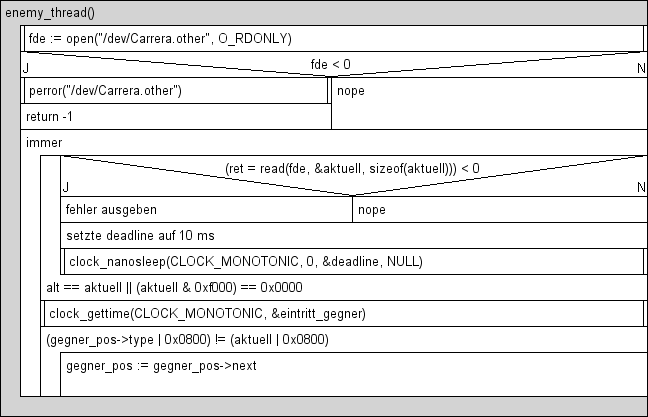
\includegraphics[width=\textwidth]{Diagramm-enemy_thread.png}
%	\caption{Funktion: \textit{void* enemy\_thread(void)}}
%\end{figure}
%\FloatBarrier

\newpage


% ================================================================================
%
%		5) Vorbereitungen und Nachbereitungen der einzelnen Teilaufgaben
%
% ================================================================================
\section{Vorbereitungen und Nachbereitungen der einzelnen Teilaufgaben}

\subsection{Termin No. 1}

\subsubsection{L\"angenberechnung der Kreuzungsbahn}
\begin{tabular}{l l}
	\textbf{Element} & \textbf{L\"ange} \\
	\hline
	Start/Ziel $ \rightarrow $ Gefahrenstelle 1 & 108 cm \\
	Gefahrenstelle 1 $ \rightarrow $ Kurve 1 & 105 cm \\
	Kurve 1 $ \rightarrow $ Kurve 2 & 91 cm \\
	Kurve 2 $ \rightarrow $ Gefahrenstelle 2 & 213 cm \\
	Gefahrenstelle 2 $ \rightarrow $ Kurve 3 & 88 cm \\
	Kurve 3 $ \rightarrow $ Kurve 4 & 112 cm \\
	Kurve 4 $ \rightarrow $ Start/Ziel & 88 cm
\end{tabular} \\

\begin{tabular}{ll}
	\textbf{Auto:} & Mercedes-Benz V8 \\
	\textbf{Gesamtl\"ange:} & 8,05 m
\end{tabular}

\subsubsection{L\"angenberechnung der Br\"uckenbahn}
\begin{tabular}{l l}
	\textbf{Element} & \textbf{L\"ange} \\
	\hline
	Start/Ziel $ \rightarrow $ Kurve 1 & 97 cm \\
	Kurve 1 $ \rightarrow $ Kurve 2 & 93 cm \\
	Kurve 2 $ \rightarrow $ Br\"uckenanfang & 79 cm \\
	Br\"uckenanfang $ \rightarrow $ Br\"uckenende & 131 cm \\
	Br\"uckenende $ \rightarrow $ Kurve 3 & 28 cm \\
	Kurve 3 $ \rightarrow $ Kurve 4 & 91 cm \\
	Kurve 4 $ \rightarrow $ Start/Ziel & 82 cm
\end{tabular} \\

\begin{tabular}{l l}
	\textbf{Auto:} & Weiss 69 \\
	\textbf{Gesamtl\"ange:} & 6,01 m
\end{tabular}

\subsubsection{Unterschied zum Gegnerthread}
Der Unterschied zum Gegnerthread liegt im 11. Bit, darin wird unterschieden, ob sich ein Fahrzeug aussen oder innen befindet, ergo m\"ussen sich der Gegner und unser Fahrzeug darin unterscheiden.

\subsection{Termin No. 2}

\subsubsection{Vorbereitung: Gegnerthread in erweiterter Form}

\code{C}{10}
\begin{lstlisting}[frame=single]
void* enemy_thread(void) {
	int fde = open("/dev/Carrera.other", O_RDONLY);
	if (fde < 0) {
		perror("/dev/Carrera.other");
		return -1;
	}

	gegner_pos = root;
	ssize_t ret;
	__u16 alt, aktuell = 0;

	if ((ret = read(fde, &alt, sizeof(alt))) < 0) {
		perror("Enemy thread: read -> alt");
		return NULL;
	}

	for (;;) {
		do {
			if ((ret = read(fde, &aktuell, sizeof(aktuell))) < 0) {
				perror("Enemy thread: read -> aktuell");
				return NULL;
			}

			struct timespec deadline;
			deadline.tv_sec = 0;
			deadline.tv_nsec = 10000000;

			clock_nanosleep(CLOCK_MONOTONIC, 0, &deadline, NULL);
		} while (alt == aktuell || (aktuell & 0xf000) == 0x0000);

		alt = aktuell;
		clock_gettime(CLOCK_MONOTONIC, &eintritt_gegner);

		while ((gegner_pos->type | 0x0800) != (aktuell | 0x0800)) {
			gegner_pos = gegner_pos->next;
		}
	}
}
\end{lstlisting}

\subsubsection{Kollisionsvermeidung}
\begin{tabular}{c | c | c | c | c}
	\textbf{Testfall} & $ t_{0} $ - 5s & $ t_{0} $ & $ t_{0} $ & \textbf{Erwartetes Ergebnis} \\
	\hline
	1 & & G \"uberf. S1 & E \"uberf. S1 & KV; nach G S2 \"uberf. hat, f\"ahrt E \\
	2 & & E \"uberf. S1 & & Keine KV \\
	3 & G \"uberf. S1 & E \"uberf. S1 & & Keine KV \\
	4 & & G \"uberf. S4 & E \"uberf. S1 & Keine KV \\
	5 & & G \"uberf. S1, bleibt stehen & E \"uberf. S1 & KV; E \"uberf. S2 max. bei $ t_{0} $ + dt +2s
\end{tabular} \\ \\ \\

\begin{tabular}{l l}
	\textbf{ABNAHME:} & \\
					& \_\_\_\_\_\_\_\_\_\_\_\_\_\_\_\_\_\_\_\_\_\_\_\_\_\_\_\_\_\_
\end{tabular}

\subsection{Termin No. 3}

\subsubsection{Vorbereitung: Ber\"ucksichtigung Streckenl\"ange}

Die Streckenl\"ange muss bei der dynamischen Geschwndigkeitsanpassung mitbeachtet werden, da damit die Geschwindigkeit anders angepasst werden kann.
Wenn ein Element sehr lang ist, lohnt es sich auf die H\"ochstgeschwindigkeit zu beschleunigen, w\"ahrend es bei einem kurzen Element weniger lohnenswert ist, da im n\"achsten ggf. wieder gebremst werden muss und damit die M\"oglichkeit besteht aus der Bahn zu fliegen.

\end{document}